\documentclass[]{article}
\usepackage{amssymb,amsmath}
\usepackage{ifxetex,ifluatex}
\ifxetex
  \usepackage{fontspec,xltxtra,xunicode}
  \defaultfontfeatures{Mapping=tex-text,Scale=MatchLowercase}
\else
  \ifluatex
    \usepackage{fontspec}
    \defaultfontfeatures{Mapping=tex-text,Scale=MatchLowercase}
  \else
    \usepackage[utf8]{inputenc}
  \fi
\fi
\usepackage{url}
\usepackage{graphicx}
% We will generate all images so they have a width \maxwidth. This means
% that they will get their normal width if they fit onto the page, but
% are scaled down if they would overflow the margins.
\makeatletter
\def\maxwidth{\ifdim\Gin@nat@width>\linewidth\linewidth
\else\Gin@nat@width\fi}
\makeatother
\let\Oldincludegraphics\includegraphics
\renewcommand{\includegraphics}[1]{\Oldincludegraphics[width=\maxwidth]{#1}}
\ifxetex
  \usepackage[setpagesize=false, % page size defined by xetex
              unicode=false, % unicode breaks when used with xetex
              xetex,
              colorlinks=true,
              linkcolor=blue]{hyperref}
\else
  \usepackage[unicode=true,
              colorlinks=true,
              linkcolor=blue]{hyperref}
\fi
\hypersetup{breaklinks=true, pdfborder={0 0 0}}
\setlength{\parindent}{0pt}
\setlength{\parskip}{6pt plus 2pt minus 1pt}
\setlength{\emergencystretch}{3em}  % prevent overfull lines
\setcounter{secnumdepth}{0}


\title{Modeling the Relationship Between Pressure and Volume of a System in a 3D Environment}
\author{Luke Carlson\\
Trevor Day School}
\renewcommand{\today}{March 11, 2013}
\maketitle

\begin{document}

\newcommand{\truncateit}


\newcommand{\scititle}


\section{Introduction}

In this lab, I set out to create a 3D simulation of ideal gas particles
in a cubic container in order to experimentally determine the pressure
of the gas based on given circumstances. From there, I planned to
explore the relationship between pressure and volume.

To produce an accurate simulation, a replication of a real world
circumstance using programming, of a gas particle it is first necessary
to understand the how the pressure can be determined.

The expected pressure of the system can be accurately modeled using the
Ideal Gas Law, which describes the characteristics of ideal gas
particles in any system. Often written as $PV=nRT$, this law displays
the relationship between Pressure, Volume, Temperature, moles of the
particle, and the universal gas constant in a system. The Ideal Gas Law
can be derived from combining three other gas laws: Boyle's Law,
Charles's Law, and Avogadro's Law.

Boyle's Law postulates that in a system with uniform temperature, the
pressure of an ideal gas is inversely proportional with volume of the
gas. Thus, the pressure times the volume is equal to a constant value in
the system, often shown as $PV = k$ (where k is the constant). Since the
constant is the same no matter the circumstances in the system, the law
can be used to relate changes in pressure or volume as
$P_{1}V_{1} = P_{2}V_{2}$ (where 1 indicates the initial and 2 is the
final state).

Charles's Law states that in a system with uniform pressure, the
temperature is inversely proportional to the volume of the container
holding the ideal gas ($V \propto T$). Since this law applies to any
variation in volume or temperature, it can be written as
$\frac{V_{1}}{T_{1}} = \frac{V_{2}}{T_{2}}$

Avogadro's Law declares that in a system with a constant temperature and
pressure, equivalent volumes of the same ideal gas will contain an equal
number of particles. Mathematically, the relationship can be shown using
$\frac{V}{n} = k$ (where k is the constant in the system).

These three laws can be combined mathematically to create
$\frac{PV}{Tn} = R$ (R is a constant in the system). When rearranged,
this creates $PV=nRT$ or the Ideal Gas Law.

To experimentally obtain a pressure through a simulation, it is
necessary to determine exactly how particles affect the pressure of a
system. Pressure is the amount of force over a specific area, also
written as $Pressure=F/A$. Force can also be described as change in
momentum over change in time: $F = \frac{\Delta p}{\Delta t}$. The
change momentum of a single particle equals its mass multiplied by its
change in velocity: ${\Delta p} = m\Delta v$. Since there is more than
one particle in a system, the entire change in momentum is the combined
change in velocities of each particle that hits the specified area.
Thus, the following formula can be used to determine total force:

\begin{center}

 $F = \frac{2m * \displaystyle\sum\limits_{0}^n v}{\Delta t}$

 \end{center}

Where $n$ is the number of collisions and $v$ is the velocity of the
particle hitting the wall. Since the change in velocity is double the
initial velocity, the 2 can be placed outside the summation along with
the mass.

Once the force has been computed using the momentum of the particles,
the pressure can then be determined with the initial formula $P = F/A$.

\section{Hypothesis}

Increasing the number of particles in the simulation will yield a
pressure closer to the actual value (determined using the Ideal Gas
Law). Furthermore, increasing the volume of a container will decrease
the pressure in the system.

\section{Method}

\subsection{Computing Pressure}

I began constructing my simulation with '3D Balls Bouncing', a project
from Open Processing, as a base. Starting off with a system that could
already handle 3D collisions of small objects inside a container was
necessary {[}see Failed Methods{]}. From there, I created small spheres
with the properties of an ideal gas. Their speed was roughly determined
on a Maxwell-Boltzman distribution and assuming that the most probable
speed ($V_{p}$) would occur the most often (calculated using the formula
$V_{p} = \sqrt{\frac{2kT}{m}}$. Next, I focused on one wall in the
container and tracked each time a particle collided with the area. I
could then compute the change in momentum over the area since I had the
masses and velocities of the particles. The simulation did not keep
track of total time since initiation, which is equivalent to time, but I
knew that aspects of the code were executed every frame. The project ran
at a fixed number of frames per second (60) so I designed this formula
to figured out the change in time:
$total\ time (seconds) = \frac{total\ frames}{frames\ per\ second}$.

I inserted that data into this formula
$F = \frac{2m * \displaystyle\sum\limits_{0}^n v}{\Delta t}$ (see
Introduction) to find the total force on the wall. To obtain the
pressure, I just divided the answer by the area of the wall.

\subsection{Testing Accuracy}

Now that I was able to compute the pressure, I could test my hypothesis
by increasing the number of particles in the system and comparing the
pressure readings. I started off with 5 particles and then tried 10, 15,
and 20 particles. I calculated the total pressure of each system once
every 5 seconds for 20 seconds.

\subsection{Assessing the Relationship Between Pressure and Volume}

The next step of my experiment involved manipulating the volume of the
container while keeping the number of particles constant. In order to do
so, I altered one line of code in the box Class:

\texttt{int boxsize = 300;}

This variable alters the dimensions of the box (currently 300x300x300
pixels). I changed the boxsize to 400, 500, and 600, and calculated the
pressure every 5 seconds for 20 seconds.


\subsection{Failed Methods}

I originally designed my own 3D collision system but it was less
efficient so a computer could not render as many particles in the
simulation. I knew that my approximation for pressure would be further
off and I also realized that it would be too time consuming to focus on
designing the base of the system when I could use open source
alternatives.

\begin{figure}[htbp]
\centering
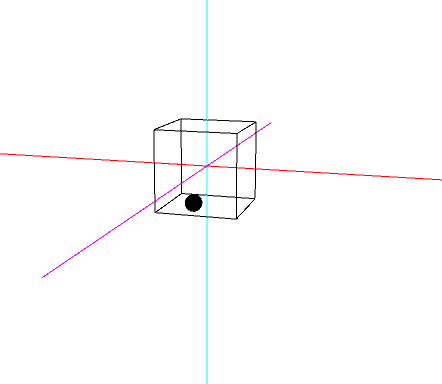
\includegraphics{pictures/failed.png}
\caption{image}
\end{figure}

\begin{figure}[htbp]
\centering
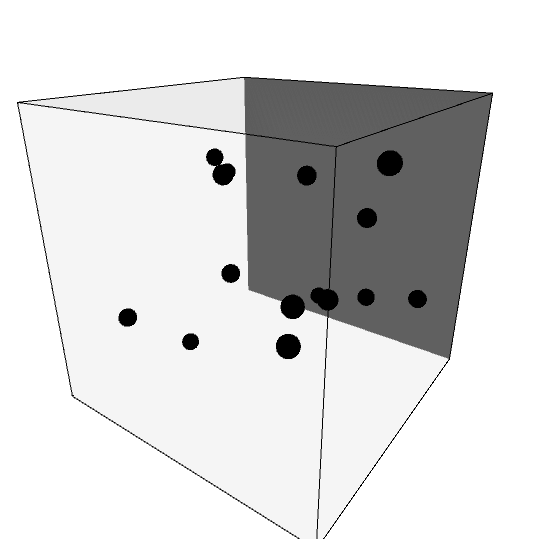
\includegraphics{pictures/simulation.png}
\caption{image}
\end{figure}

\section{Results}
\begin{table}[ht]
\caption{Estimating Pressure}
\centering 
\begin{tabular}{c c c c c c} 
\hline\hline 
Number of Particles & First Pressure Reading & Second & Third & Fourth�& Average \\
\hline 
5 & 1.98E-06 & 1.33E-06 & 1.14E-06 & 9.63E-07 & 1.35E-06 \\ 
10 & 4.13E-06 & 3.74E-06 & 4.14E-06 & 4.56E-06 & 4.14E-06 \\ 
15 & 6.94E-06 & 6.96E-06 & 6.43E-06 & 6.55E-06 & 6.72E-06 \\ 
20 & 7.00E-06 & 6.54E-06 & 6.50E-06 & 7.43E-06 & 6.87E-06 \\
\hline 
\end{tabular}
\label{table:estpress} 
\end{table}

\begin{table}
\begin{tabular}{| l | l | l | l | l | l |}
Dimensions of Box (px) & First Pressure Reading & Second�� & Third��� & Fourth�� & Average� \\ \hline
300 & 7.00E-06 & 6.54E-06 & 6.50E-06 & 7.43E-06 & 6.87E-06 \\ 
400 & 4.68E-06 & 4.42E-06 & 4.28E-06 & 4.11E-06 & 4.37E-06 \\ 
500 & 4.15E-06 & 3.42E-06 & 3.21E-06 & 3.26E-06 & 3.51E-06 \\ 
600 & 3.48E-06 & 3.31E-06 & 2.89E-06 & 2.73E-06 & 3.10E-06 \\
\end{tabular}
\end{table}

\section{Discussion}

Concisely state the results and what I learned

\section{Improvements}

\begin{enumerate}
\item
  Since the simulation could not handle a large number of particles, I
  had to resort to using an unrealistically low number of particles
  (e.g. 5 particles vs $5 x 10^{23}$).

  \begin{enumerate}
  \item
    This also meant that my Maxwell--Boltzmann distribution would not be
    as precise because if a particle obtained a truely outlier speed, it
    would greatly affect the results
  \end{enumerate}
\item
  Add more improvements \ldots{}
\end{enumerate}
\section{Bibliography}

\begin{itemize}
\item
  "Maxwell Speed Distribution Directly from Boltzmann Distribution."
  Development of Maxwell Distribution. N.p., n.d. Web. 07 Mar.
  2013.\textless{}\url{http://hyperphysics.phy-astr.gsu.edu/%E2%80%8Chbase/kinetic/maxspe.html}\textgreater{}.
\item
  "Language Reference (API) Processing 2." Language Reference (API)
  Processing 2. N.p., n.d. Web. 07 Mar. 2013.
  \textless{}\url{http://processing.org/reference}\textgreater{}.
\item
  "3D Balls Bouncing- OpenProcessing." 3D Balls Bouncing-
  OpenProcessing. N.p., n.d. Web. 07 Mar. 2013.
  \textless{}\url{http://www.openprocessing.org/sketch/20136}\textgreater{}.
\item
  "Kinetic Theory." Wikipedia. Wikimedia Foundation, 03 Apr. 2013. Web.
  07 Mar. 2013.
\item
  "The Distribution of Molecular Speeds." ChemEd. University of
  Wisconsin, n.d. Web. 10 Mar. 2013.
  \textless{}\url{http://chemed.chem.wisc.edu/chempaths/GenChem-Textbook/Kinetic-Theory-of-Gases-The-Distribution-of-Molecular-Speeds-941.html}\textgreater{}.
\item
  "Including Graphics in a LaTeX Document." Including Graphics in a
  LaTeX Document. University Of Colorado Boulder, n.d. Web. 10 Mar.
  2013.
  \textless{}\url{http://amath.colorado.edu/documentation/LaTeX/reference/figures.html}\textgreater{}.
\end{itemize}

\end{document}

